\documentclass{article} % For LaTeX2e
\usepackage{iclr2023_conference, times}

% --- Default packages --- 
% Optional math commands from https://github.com/goodfeli/dlbook_notation.
%%%%% NEW MATH DEFINITIONS %%%%%

\usepackage{amsmath,amsfonts,bm}

% Mark sections of captions for referring to divisions of figures
\newcommand{\figleft}{{\em (Left)}}
\newcommand{\figcenter}{{\em (Center)}}
\newcommand{\figright}{{\em (Right)}}
\newcommand{\figtop}{{\em (Top)}}
\newcommand{\figbottom}{{\em (Bottom)}}
\newcommand{\captiona}{{\em (a)}}
\newcommand{\captionb}{{\em (b)}}
\newcommand{\captionc}{{\em (c)}}
\newcommand{\captiond}{{\em (d)}}

% Highlight a newly defined term
\newcommand{\newterm}[1]{{\bf #1}}


% Figure reference, lower-case.
\def\figref#1{figure~\ref{#1}}
% Figure reference, capital. For start of sentence
\def\Figref#1{Figure~\ref{#1}}
\def\twofigref#1#2{figures \ref{#1} and \ref{#2}}
\def\quadfigref#1#2#3#4{figures \ref{#1}, \ref{#2}, \ref{#3} and \ref{#4}}
% Section reference, lower-case.
\def\secref#1{section~\ref{#1}}
% Section reference, capital.
\def\Secref#1{Section~\ref{#1}}
% Reference to two sections.
\def\twosecrefs#1#2{sections \ref{#1} and \ref{#2}}
% Reference to three sections.
\def\secrefs#1#2#3{sections \ref{#1}, \ref{#2} and \ref{#3}}
% Reference to an equation, lower-case.
\def\eqref#1{equation~\ref{#1}}
% Reference to an equation, upper case
\def\Eqref#1{Equation~\ref{#1}}
% A raw reference to an equation---avoid using if possible
\def\plaineqref#1{\ref{#1}}
% Reference to a chapter, lower-case.
\def\chapref#1{chapter~\ref{#1}}
% Reference to an equation, upper case.
\def\Chapref#1{Chapter~\ref{#1}}
% Reference to a range of chapters
\def\rangechapref#1#2{chapters\ref{#1}--\ref{#2}}
% Reference to an algorithm, lower-case.
\def\algref#1{algorithm~\ref{#1}}
% Reference to an algorithm, upper case.
\def\Algref#1{Algorithm~\ref{#1}}
\def\twoalgref#1#2{algorithms \ref{#1} and \ref{#2}}
\def\Twoalgref#1#2{Algorithms \ref{#1} and \ref{#2}}
% Reference to a part, lower case
\def\partref#1{part~\ref{#1}}
% Reference to a part, upper case
\def\Partref#1{Part~\ref{#1}}
\def\twopartref#1#2{parts \ref{#1} and \ref{#2}}

\def\ceil#1{\lceil #1 \rceil}
\def\floor#1{\lfloor #1 \rfloor}
\def\1{\bm{1}}
\newcommand{\train}{\mathcal{D}}
\newcommand{\valid}{\mathcal{D_{\mathrm{valid}}}}
\newcommand{\test}{\mathcal{D_{\mathrm{test}}}}

\def\eps{{\epsilon}}


% Random variables
\def\reta{{\textnormal{$\eta$}}}
\def\ra{{\textnormal{a}}}
\def\rb{{\textnormal{b}}}
\def\rc{{\textnormal{c}}}
\def\rd{{\textnormal{d}}}
\def\re{{\textnormal{e}}}
\def\rf{{\textnormal{f}}}
\def\rg{{\textnormal{g}}}
\def\rh{{\textnormal{h}}}
\def\ri{{\textnormal{i}}}
\def\rj{{\textnormal{j}}}
\def\rk{{\textnormal{k}}}
\def\rl{{\textnormal{l}}}
% rm is already a command, just don't name any random variables m
\def\rn{{\textnormal{n}}}
\def\ro{{\textnormal{o}}}
\def\rp{{\textnormal{p}}}
\def\rq{{\textnormal{q}}}
\def\rr{{\textnormal{r}}}
\def\rs{{\textnormal{s}}}
\def\rt{{\textnormal{t}}}
\def\ru{{\textnormal{u}}}
\def\rv{{\textnormal{v}}}
\def\rw{{\textnormal{w}}}
\def\rx{{\textnormal{x}}}
\def\ry{{\textnormal{y}}}
\def\rz{{\textnormal{z}}}

% Random vectors
\def\rvepsilon{{\mathbf{\epsilon}}}
\def\rvtheta{{\mathbf{\theta}}}
\def\rva{{\mathbf{a}}}
\def\rvb{{\mathbf{b}}}
\def\rvc{{\mathbf{c}}}
\def\rvd{{\mathbf{d}}}
\def\rve{{\mathbf{e}}}
\def\rvf{{\mathbf{f}}}
\def\rvg{{\mathbf{g}}}
\def\rvh{{\mathbf{h}}}
\def\rvu{{\mathbf{i}}}
\def\rvj{{\mathbf{j}}}
\def\rvk{{\mathbf{k}}}
\def\rvl{{\mathbf{l}}}
\def\rvm{{\mathbf{m}}}
\def\rvn{{\mathbf{n}}}
\def\rvo{{\mathbf{o}}}
\def\rvp{{\mathbf{p}}}
\def\rvq{{\mathbf{q}}}
\def\rvr{{\mathbf{r}}}
\def\rvs{{\mathbf{s}}}
\def\rvt{{\mathbf{t}}}
\def\rvu{{\mathbf{u}}}
\def\rvv{{\mathbf{v}}}
\def\rvw{{\mathbf{w}}}
\def\rvx{{\mathbf{x}}}
\def\rvy{{\mathbf{y}}}
\def\rvz{{\mathbf{z}}}

% Elements of random vectors
\def\erva{{\textnormal{a}}}
\def\ervb{{\textnormal{b}}}
\def\ervc{{\textnormal{c}}}
\def\ervd{{\textnormal{d}}}
\def\erve{{\textnormal{e}}}
\def\ervf{{\textnormal{f}}}
\def\ervg{{\textnormal{g}}}
\def\ervh{{\textnormal{h}}}
\def\ervi{{\textnormal{i}}}
\def\ervj{{\textnormal{j}}}
\def\ervk{{\textnormal{k}}}
\def\ervl{{\textnormal{l}}}
\def\ervm{{\textnormal{m}}}
\def\ervn{{\textnormal{n}}}
\def\ervo{{\textnormal{o}}}
\def\ervp{{\textnormal{p}}}
\def\ervq{{\textnormal{q}}}
\def\ervr{{\textnormal{r}}}
\def\ervs{{\textnormal{s}}}
\def\ervt{{\textnormal{t}}}
\def\ervu{{\textnormal{u}}}
\def\ervv{{\textnormal{v}}}
\def\ervw{{\textnormal{w}}}
\def\ervx{{\textnormal{x}}}
\def\ervy{{\textnormal{y}}}
\def\ervz{{\textnormal{z}}}

% Random matrices
\def\rmA{{\mathbf{A}}}
\def\rmB{{\mathbf{B}}}
\def\rmC{{\mathbf{C}}}
\def\rmD{{\mathbf{D}}}
\def\rmE{{\mathbf{E}}}
\def\rmF{{\mathbf{F}}}
\def\rmG{{\mathbf{G}}}
\def\rmH{{\mathbf{H}}}
\def\rmI{{\mathbf{I}}}
\def\rmJ{{\mathbf{J}}}
\def\rmK{{\mathbf{K}}}
\def\rmL{{\mathbf{L}}}
\def\rmM{{\mathbf{M}}}
\def\rmN{{\mathbf{N}}}
\def\rmO{{\mathbf{O}}}
\def\rmP{{\mathbf{P}}}
\def\rmQ{{\mathbf{Q}}}
\def\rmR{{\mathbf{R}}}
\def\rmS{{\mathbf{S}}}
\def\rmT{{\mathbf{T}}}
\def\rmU{{\mathbf{U}}}
\def\rmV{{\mathbf{V}}}
\def\rmW{{\mathbf{W}}}
\def\rmX{{\mathbf{X}}}
\def\rmY{{\mathbf{Y}}}
\def\rmZ{{\mathbf{Z}}}

% Elements of random matrices
\def\ermA{{\textnormal{A}}}
\def\ermB{{\textnormal{B}}}
\def\ermC{{\textnormal{C}}}
\def\ermD{{\textnormal{D}}}
\def\ermE{{\textnormal{E}}}
\def\ermF{{\textnormal{F}}}
\def\ermG{{\textnormal{G}}}
\def\ermH{{\textnormal{H}}}
\def\ermI{{\textnormal{I}}}
\def\ermJ{{\textnormal{J}}}
\def\ermK{{\textnormal{K}}}
\def\ermL{{\textnormal{L}}}
\def\ermM{{\textnormal{M}}}
\def\ermN{{\textnormal{N}}}
\def\ermO{{\textnormal{O}}}
\def\ermP{{\textnormal{P}}}
\def\ermQ{{\textnormal{Q}}}
\def\ermR{{\textnormal{R}}}
\def\ermS{{\textnormal{S}}}
\def\ermT{{\textnormal{T}}}
\def\ermU{{\textnormal{U}}}
\def\ermV{{\textnormal{V}}}
\def\ermW{{\textnormal{W}}}
\def\ermX{{\textnormal{X}}}
\def\ermY{{\textnormal{Y}}}
\def\ermZ{{\textnormal{Z}}}

% Vectors
\def\vzero{{\bm{0}}}
\def\vone{{\bm{1}}}
\def\vmu{{\bm{\mu}}}
\def\vtheta{{\bm{\theta}}}
\def\va{{\bm{a}}}
\def\vb{{\bm{b}}}
\def\vc{{\bm{c}}}
\def\vd{{\bm{d}}}
\def\ve{{\bm{e}}}
\def\vf{{\bm{f}}}
\def\vg{{\bm{g}}}
\def\vh{{\bm{h}}}
\def\vi{{\bm{i}}}
\def\vj{{\bm{j}}}
\def\vk{{\bm{k}}}
\def\vl{{\bm{l}}}
\def\vm{{\bm{m}}}
\def\vn{{\bm{n}}}
\def\vo{{\bm{o}}}
\def\vp{{\bm{p}}}
\def\vq{{\bm{q}}}
\def\vr{{\bm{r}}}
\def\vs{{\bm{s}}}
\def\vt{{\bm{t}}}
\def\vu{{\bm{u}}}
\def\vv{{\bm{v}}}
\def\vw{{\bm{w}}}
\def\vx{{\bm{x}}}
\def\vy{{\bm{y}}}
\def\vz{{\bm{z}}}

% Elements of vectors
\def\evalpha{{\alpha}}
\def\evbeta{{\beta}}
\def\evepsilon{{\epsilon}}
\def\evlambda{{\lambda}}
\def\evomega{{\omega}}
\def\evmu{{\mu}}
\def\evpsi{{\psi}}
\def\evsigma{{\sigma}}
\def\evtheta{{\theta}}
\def\eva{{a}}
\def\evb{{b}}
\def\evc{{c}}
\def\evd{{d}}
\def\eve{{e}}
\def\evf{{f}}
\def\evg{{g}}
\def\evh{{h}}
\def\evi{{i}}
\def\evj{{j}}
\def\evk{{k}}
\def\evl{{l}}
\def\evm{{m}}
\def\evn{{n}}
\def\evo{{o}}
\def\evp{{p}}
\def\evq{{q}}
\def\evr{{r}}
\def\evs{{s}}
\def\evt{{t}}
\def\evu{{u}}
\def\evv{{v}}
\def\evw{{w}}
\def\evx{{x}}
\def\evy{{y}}
\def\evz{{z}}

% Matrix
\def\mA{{\bm{A}}}
\def\mB{{\bm{B}}}
\def\mC{{\bm{C}}}
\def\mD{{\bm{D}}}
\def\mE{{\bm{E}}}
\def\mF{{\bm{F}}}
\def\mG{{\bm{G}}}
\def\mH{{\bm{H}}}
\def\mI{{\bm{I}}}
\def\mJ{{\bm{J}}}
\def\mK{{\bm{K}}}
\def\mL{{\bm{L}}}
\def\mM{{\bm{M}}}
\def\mN{{\bm{N}}}
\def\mO{{\bm{O}}}
\def\mP{{\bm{P}}}
\def\mQ{{\bm{Q}}}
\def\mR{{\bm{R}}}
\def\mS{{\bm{S}}}
\def\mT{{\bm{T}}}
\def\mU{{\bm{U}}}
\def\mV{{\bm{V}}}
\def\mW{{\bm{W}}}
\def\mX{{\bm{X}}}
\def\mY{{\bm{Y}}}
\def\mZ{{\bm{Z}}}
\def\mBeta{{\bm{\beta}}}
\def\mPhi{{\bm{\Phi}}}
\def\mLambda{{\bm{\Lambda}}}
\def\mSigma{{\bm{\Sigma}}}

% Tensor
\DeclareMathAlphabet{\mathsfit}{\encodingdefault}{\sfdefault}{m}{sl}
\SetMathAlphabet{\mathsfit}{bold}{\encodingdefault}{\sfdefault}{bx}{n}
\newcommand{\tens}[1]{\bm{\mathsfit{#1}}}
\def\tA{{\tens{A}}}
\def\tB{{\tens{B}}}
\def\tC{{\tens{C}}}
\def\tD{{\tens{D}}}
\def\tE{{\tens{E}}}
\def\tF{{\tens{F}}}
\def\tG{{\tens{G}}}
\def\tH{{\tens{H}}}
\def\tI{{\tens{I}}}
\def\tJ{{\tens{J}}}
\def\tK{{\tens{K}}}
\def\tL{{\tens{L}}}
\def\tM{{\tens{M}}}
\def\tN{{\tens{N}}}
\def\tO{{\tens{O}}}
\def\tP{{\tens{P}}}
\def\tQ{{\tens{Q}}}
\def\tR{{\tens{R}}}
\def\tS{{\tens{S}}}
\def\tT{{\tens{T}}}
\def\tU{{\tens{U}}}
\def\tV{{\tens{V}}}
\def\tW{{\tens{W}}}
\def\tX{{\tens{X}}}
\def\tY{{\tens{Y}}}
\def\tZ{{\tens{Z}}}


% Graph
\def\gA{{\mathcal{A}}}
\def\gB{{\mathcal{B}}}
\def\gC{{\mathcal{C}}}
\def\gD{{\mathcal{D}}}
\def\gE{{\mathcal{E}}}
\def\gF{{\mathcal{F}}}
\def\gG{{\mathcal{G}}}
\def\gH{{\mathcal{H}}}
\def\gI{{\mathcal{I}}}
\def\gJ{{\mathcal{J}}}
\def\gK{{\mathcal{K}}}
\def\gL{{\mathcal{L}}}
\def\gM{{\mathcal{M}}}
\def\gN{{\mathcal{N}}}
\def\gO{{\mathcal{O}}}
\def\gP{{\mathcal{P}}}
\def\gQ{{\mathcal{Q}}}
\def\gR{{\mathcal{R}}}
\def\gS{{\mathcal{S}}}
\def\gT{{\mathcal{T}}}
\def\gU{{\mathcal{U}}}
\def\gV{{\mathcal{V}}}
\def\gW{{\mathcal{W}}}
\def\gX{{\mathcal{X}}}
\def\gY{{\mathcal{Y}}}
\def\gZ{{\mathcal{Z}}}

% Sets
\def\sA{{\mathbb{A}}}
\def\sB{{\mathbb{B}}}
\def\sC{{\mathbb{C}}}
\def\sD{{\mathbb{D}}}
% Don't use a set called E, because this would be the same as our symbol
% for expectation.
\def\sF{{\mathbb{F}}}
\def\sG{{\mathbb{G}}}
\def\sH{{\mathbb{H}}}
\def\sI{{\mathbb{I}}}
\def\sJ{{\mathbb{J}}}
\def\sK{{\mathbb{K}}}
\def\sL{{\mathbb{L}}}
\def\sM{{\mathbb{M}}}
\def\sN{{\mathbb{N}}}
\def\sO{{\mathbb{O}}}
\def\sP{{\mathbb{P}}}
\def\sQ{{\mathbb{Q}}}
\def\sR{{\mathbb{R}}}
\def\sS{{\mathbb{S}}}
\def\sT{{\mathbb{T}}}
\def\sU{{\mathbb{U}}}
\def\sV{{\mathbb{V}}}
\def\sW{{\mathbb{W}}}
\def\sX{{\mathbb{X}}}
\def\sY{{\mathbb{Y}}}
\def\sZ{{\mathbb{Z}}}

% Entries of a matrix
\def\emLambda{{\Lambda}}
\def\emA{{A}}
\def\emB{{B}}
\def\emC{{C}}
\def\emD{{D}}
\def\emE{{E}}
\def\emF{{F}}
\def\emG{{G}}
\def\emH{{H}}
\def\emI{{I}}
\def\emJ{{J}}
\def\emK{{K}}
\def\emL{{L}}
\def\emM{{M}}
\def\emN{{N}}
\def\emO{{O}}
\def\emP{{P}}
\def\emQ{{Q}}
\def\emR{{R}}
\def\emS{{S}}
\def\emT{{T}}
\def\emU{{U}}
\def\emV{{V}}
\def\emW{{W}}
\def\emX{{X}}
\def\emY{{Y}}
\def\emZ{{Z}}
\def\emSigma{{\Sigma}}

% entries of a tensor
% Same font as tensor, without \bm wrapper
\newcommand{\etens}[1]{\mathsfit{#1}}
\def\etLambda{{\etens{\Lambda}}}
\def\etA{{\etens{A}}}
\def\etB{{\etens{B}}}
\def\etC{{\etens{C}}}
\def\etD{{\etens{D}}}
\def\etE{{\etens{E}}}
\def\etF{{\etens{F}}}
\def\etG{{\etens{G}}}
\def\etH{{\etens{H}}}
\def\etI{{\etens{I}}}
\def\etJ{{\etens{J}}}
\def\etK{{\etens{K}}}
\def\etL{{\etens{L}}}
\def\etM{{\etens{M}}}
\def\etN{{\etens{N}}}
\def\etO{{\etens{O}}}
\def\etP{{\etens{P}}}
\def\etQ{{\etens{Q}}}
\def\etR{{\etens{R}}}
\def\etS{{\etens{S}}}
\def\etT{{\etens{T}}}
\def\etU{{\etens{U}}}
\def\etV{{\etens{V}}}
\def\etW{{\etens{W}}}
\def\etX{{\etens{X}}}
\def\etY{{\etens{Y}}}
\def\etZ{{\etens{Z}}}

% The true underlying data generating distribution
\newcommand{\pdata}{p_{\rm{data}}}
% The empirical distribution defined by the training set
\newcommand{\ptrain}{\hat{p}_{\rm{data}}}
\newcommand{\Ptrain}{\hat{P}_{\rm{data}}}
% The model distribution
\newcommand{\pmodel}{p_{\rm{model}}}
\newcommand{\Pmodel}{P_{\rm{model}}}
\newcommand{\ptildemodel}{\tilde{p}_{\rm{model}}}
% Stochastic autoencoder distributions
\newcommand{\pencode}{p_{\rm{encoder}}}
\newcommand{\pdecode}{p_{\rm{decoder}}}
\newcommand{\precons}{p_{\rm{reconstruct}}}

\newcommand{\laplace}{\mathrm{Laplace}} % Laplace distribution

\newcommand{\E}{\mathbb{E}}
\newcommand{\Ls}{\mathcal{L}}
\newcommand{\R}{\mathbb{R}}
\newcommand{\emp}{\tilde{p}}
\newcommand{\lr}{\alpha}
\newcommand{\reg}{\lambda}
\newcommand{\rect}{\mathrm{rectifier}}
\newcommand{\softmax}{\mathrm{softmax}}
\newcommand{\sigmoid}{\sigma}
\newcommand{\softplus}{\zeta}
\newcommand{\KL}{D_{\mathrm{KL}}}
\newcommand{\Var}{\mathrm{Var}}
\newcommand{\standarderror}{\mathrm{SE}}
\newcommand{\Cov}{\mathrm{Cov}}
% Wolfram Mathworld says $L^2$ is for function spaces and $\ell^2$ is for vectors
% But then they seem to use $L^2$ for vectors throughout the site, and so does
% wikipedia.
\newcommand{\normlzero}{L^0}
\newcommand{\normlone}{L^1}
\newcommand{\normltwo}{L^2}
\newcommand{\normlp}{L^p}
\newcommand{\normmax}{L^\infty}

\newcommand{\parents}{Pa} % See usage in notation.tex. Chosen to match Daphne's book.

\DeclareMathOperator*{\argmax}{arg\,max}
\DeclareMathOperator*{\argmin}{arg\,min}

\DeclareMathOperator{\sign}{sign}
\DeclareMathOperator{\Tr}{Tr}
\let\ab\allowbreak

\usepackage{hyperref}
\usepackage{url}

% --- Custom packages --- 
\usepackage{graphicx}


\title{Title \\ Subtitle}

% Authors must not appear in the submitted version. They should be hidden
% as long as the \iclrfinalcopy macro remains commented out below.
% Non-anonymous submissions will be rejected without review.

\author{%
    Joseph Lavond \& Yao Li  \\
    Department of Statistics and Operations Research \\
    University of North Carolina at Chapel Hill \\
    Chapel Hill, NC 27514, USA \\
    \texttt{\{jlavond, yaoli\}@unc.email.edu} \\
    %
    \And
    Minhao Cheng \\
    Computer Science and Engineering \\
    Hong Kong University of Science and Technology \\
    Clear Water Bay, Hong Kong \\
    \texttt{minhaocheng@ust.hk}
}

% The \author macro works with any number of authors. There are two commands
% used to separate the names and addresses of multiple authors: \And and \AND.
%
% Using \And between authors leaves it to \LaTeX{} to determine where to break
% the lines. Using \AND forces a linebreak at that point. So, if \LaTeX{}
% puts 3 of 4 authors names on the first line, and the last on the second
% line, try using \AND instead of \And before the third author name.

\newcommand{\fix}{\marginpar{FIX}}
\newcommand{\new}{\marginpar{NEW}}

%\iclrfinalcopy % Uncomment for camera-ready version, but NOT for submission.
\begin{document}


\maketitle

\begin{abstract}
Abstract text here.
\end{abstract}

% ----- Content -----
\section{Introduction}

Federated learning is a potential solution to constructing a machine learning model from several local data sources that cannot be exchanged or aggregated. These restrictions are essential in areas where data privacy or security is critical such as healthcare and defense. However, federated learning is also valuable to companies that can shift much of the computing workload to local devices instead. Furthermore, the local datasets are not required to be independent and identically distributed. Hence, a shared robust global model is desirable and, in many cases, cannot be produced without some form of collaborative learning.

At a high level, federated learning is an iterative procedure of rounds until it meets some termination criteria. These rounds consist of sending the global model to users and selecting a subset of users to update the global model. Those chosen users train their local copy of the model, and their resulting models are communicated back and aggregated in some manner to create a new global model. Typically, the final local model's gradients or weights are transmitted back to ensure privacy or keep the necessary resources minimal. 

Concerns have arisen that the lack of control or knowledge regarding the local training procedure could allow a user, with malicious intent, to create an update that compromises the global model for all future users. An example of such harm is a backdoor attack, where training attempt to get a model to associate a given manipulation of the input data, known as a trigger, with a particular outcome. Recent work, such as by \cite{stamp-invisible}., creates backdoor triggers that are not detectable in the data by human or computer vision. However, in federated learning, only the resulting model gradients or weights are communicated, so there is potentially no need to hide the trigger in the data. Furthermore, without access to leverage user input data, there is less information available to help detect and prevent such malicious intent.

Our contribution to federated learning is establishing defense criteria for federated learning, which is effective against multiple attackers, model scaling, and attacks before global model convergence. Furthermore, our threshold still allows many regular users to update the global model, resulting in little to no performance degradation and requiring only a minimal increase in computational resources or time.

%
\section{Related Work}


%
\section{Method}

We must assume that malicious users cannot compromise the aggregation method used to update the global model other than modify their returned local model weights. However, we make the additional assumption that there exists one user who we can be confident is trustworthy to place in charge of gate-keeping the global model for updates. That user will evaluate incoming model weights and determine whether each contribution is allowed to participate in the FedAvg procedure, detailed in \cite{fedavg}. Their decision will be made independently of other users and thus will not violate any data privacy or security concerns.

Our method attempts to detect unusually distributed output layers of the returning user models from this single trusted user. Moving forward, we intend to refer to this single trusted user as the validation user. In each communication round, this user completes the following additional steps to create an estimated upper bound for the most considerable change a non-malicious user can make to the output layer of the global model:
\begin{enumerate}
    \item The validation user computes and stores a forward pass of the current global model on their local data.
    \item They perform local training of the global model and then calculate and store a forward pass of their data on their updated model.
    \item The user determines a defense threshold from these former forward passes by computing the distance between the output layers of the original and updated model.
    \item When the subset of K users submits their updated model weights, each has a forward pass performed on the validation user's local data and the distance calculated between the previous global model and their locally trained models. If their distance exceeds the proposed round threshold, we omit their submitted model from participating in the update. 
\end{enumerate}

Only step 2 has a high relative computation cost as local training will require gradient calculations. However, users often train on local compute resources in the Federated Learning setting. Therefore, the validation user will do this step simultaneously with the local training of other users. The only additional steps not being done during existing parts of Federated Learning are forward passes, which are less complex and quickly accelerated by modern computing architectures.

In addition, the computation of the distance between output layer distributions of the models is also efficient. We avoid distributional assumptions on the output layer by using each class's empirical cumulative distribution function (CDF) \footnote{$\hat F_x(t) = \dfrac{\sum_i I(x_i \leq t)}{\testrm{length}(x)}$}, and we measure the class conditional distributional difference using the Kolmogorov-Smirnov (KS) distance \footnote{$KS(F_1, F_2) = \sup_t | F_1(t) - F_2(t) |$}. Using the property that the empirical CDFs are step functions, note that the KS distance between the empirical CDFs only needs to be computed for each of the values of the class scores on the local user's data for both the global and trusted user's updated model. Furthermore, this computation is embarrassingly parallelizable, meaning that each value can be computed separately, without communication, between the calculations. 


Thus, for each user in the subset of K users and the validation user, the additional steps to Federated Learning result in a vector of KS distances, $\rvd$, one for each class. Again, recall that we intend to determine the most considerable possible change that a non-malicious user could contribute and exclude all users from participating in the update of the global model that exceeds such a threshold. Hence, we want to estimate the most prominent possible KS distance for any class for use as a cutoff. We operate under the assumption that the class distances are Uniform on $[0, b_c]$ for each class c, where $b_c$ is our estimate for the maximum possible change to the output layer of class c through local training by a non-malicious user. Note that this representation is conservative for other uni-modal distributions, as the Uniform distribution has the most considerable variance of uni-modal distributions over the same support. Therefore, we aim to estimate and use the maximum of $b_c$, the maximal benign change to any class, as a cutoff for returning user models. Recall that doubling a single sample from a Uniform distribution is an unbiased estimate for the maximum of the distribution. Since the class distances are Uniform, and we have a single sample for each communication round, doubling the KS distances for the validation user is an unbiased estimate for each $b_c$, and we will use $\max_c (2 * d_c)$, where $\rvd$ is the trusted user's KS distances. Note that we are not claiming that our threshold is unbiased for $\max_c (b_c)$. However, we will demonstrate its usefulness after a few modifications to address the following concerns that we observe with the original cutoff:
\begin{enumerate}
    \item There is extreme instability round-to-round in our threshold. A lucky malicious user can get past a large cutoff for that round due to instability.
    \item In early communication rounds, the cutoff rapidly decreases as the model starts making connections between inputs and output classes. Malicious users have a large opportunity to impact the model at the beginning of Federated Learning.
    \item The threshold values depend heavily on the distribution of class labels for the validated user.
\end{enumerate}
Our final threshold includes the following solutions to the above problems.

%
\subsection{Global Min-Mean Threshold}

We needed to develop a stable cutoff that is a meaningful estimate of the maximum distance a benign user can submit for a given round. By assuming that certain consecutive rounds have the same value of $b_c$, we can use instead the running average of the cutoff across rounds which would have the same expected value with reduced variability. Note that we can view this average as smoothing across all previous values with equal weight. Although smoothing solves our instability problem, smoothing methods exacerbate the second problem, where $b_c$ tends to decrease rapidly over the first few communication rounds. When $b_c$ decreases, we do not wish to use any previous communication rounds for our threshold. Our solution is to use as our cutoff the running mean since the lowest observed value (Global Min-Mean) of the maximum class distance for the validated user. Our solution quickly adapts to decreasing values of $b_c$. As $b_c$ shrinks, we observe new global minimums, and the start of the threshold is reset. In addition, when $b_c$ stabilizes, the averaging smooths our cutoff, keeping lucky malicious users from getting past a volatile threshold.

%
\subsection{Entropy Based Distance Scaling}

In some cases, having a trusted user with a balanced distribution of class labels may not be possible. The ability to construct a cutoff from unbalanced data helps when data cannot be collected and avoids any data privacy or security issues associated with sharing one's local class labels with other users. From initial experimentation, we saw that either over or under-represented classes result in larger KS values than benign users with a balanced distribution of class labels. From information theory, Shannon Entropy \footnote{For a discrete random variable $\rvx$ with levels c, entropy is defined $H(x) = - \sum_c P(x_c) \log P(x_c)$} is one such measure of diversity. Note that entropy is maximized when class labels are uniformly distributed. Consider instead each class's contribution towards entropy, $H_c(x) = - P(x_c) \log P(x_c)$, and let D be the total number of classes. We propose scaling the distance between global and updated models for each class for multi-class classification problems by the following factor $S_c$, before computing the maximum and multiplying by two. Note that $S$, the collection of $S_c$, only needs to be computed once, as it depends on the local user's class label distribution and does not depend on the distance values each round.

\begin{align}
    y_c &= \min \left( x_c, \dfrac{1}{e} \right) \\
    z_c &= \min \left( \dfrac{P(y_c) \ln \left( P(y_c) \right)}{\dfrac{1}{D} \ln \left( \dfrac{1}{D} \right)}, 2 \right) \\
    S_c &= 1 - | 1 - z_c |    
\end{align}

\begin{figure}[h]
    \centering
    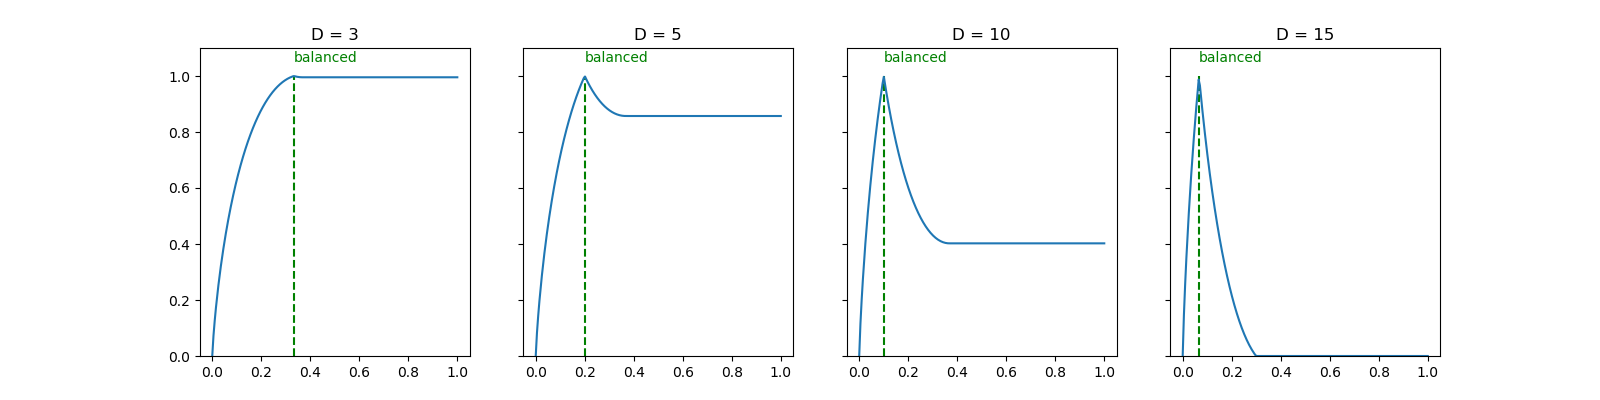
\includegraphics[width=\textwidth]{article/99_visuals/scaling.png}
    \caption{Entropy Based Scaling ($S_c$) for Several Size Classification Problems}
    \label{fig:scaling}
\end{figure}

See Figure \ref{fig:scaling} for $S_c(x)$ plotted as a function of the class proportions for several values of $D$, the total number of classes. Observe the following  properties:
\begin{enumerate}
    \item Scaling is between 0 and 1, and there is no scaling when a given class is balanced
    \item Under-represented classes are scaled down to zero
    \item For many-class classification problems, we are less trusting of an over-represented class as we have more potential classes for at least one to be approximately balanced.
\end{enumerate}

We believe further research is needed regarding extremely imbalanced edge cases. However, we propose this scaling as a remedy for reasonably imbalanced data, demonstrating its promising effectiveness in our experimentation.

\section{EXPERIMENTS}

%
\subsection{Setting}

We start by giving further specifications regarding the federated learning environment. Our interest is training a global model over M communication rounds with N users. Each iteration randomly selects K users, using a specified proportion of the total users, to participate in the model update. After local training, the next global model is the average of returning model weights by the FedAvg procedure. 

To produce local datasets that do not have to be independent and identically distributed, we sample from any training data set using a Dirichlet distribution with specified parameter alpha. The Dirichlet sample determines the proportion of each class included in that user's dataset. Larger values of alpha produce more balanced class distributions. We separately control alpha for benign, malicious, and validation users. Our experiments use the CIFAR-10 dataset, which consists of 60000 32x32 color images in 10 classes, with 6000 images per class. We use the test set of 10000 images, with 500 images per class, for model evaluation. Our experiments use the ResNet18 model architecture, a state-of-the-ark off-the-shelf classifier for object recognition, initially proposed in \cite{resnet}. 

We assume that all users, including malicious, have complete control over all aspects of local training, such as learning rate, the number of epochs, and the model weights they return. The malicious users will poison a given proportion of their local data by adding their backdoor trigger to the input and changing the training label to that of the target class. They intend for the model to associate the trigger with the target class and hence have the future global model identify any input with the trigger as belonging to the target class. For simplicity, we select two main sets of training hyperparameters for benign and malicious users. 

To further show the effectiveness of our method, we choose an unrealistic and unreasonable strong attack setting. We force all malicious users to be included in the subset of users to update the global model each round after the start of the backdoor attack. Note that the selection of random users is a defense against malicious users by making it difficult for them to update the global model repeatedly. Additionally, we do not allow the validation user, a guaranteed benign user, to participate in any global model updates. We make these decisions to show the ability of our threshold to prevent even strong backdoor attacks against the global model. 

For global model evaluation, we split the test set, added the backdoor trigger to half, and removed any target class observations from that half's data. We use classification accuracy from the first half to measure model success, and the proportion of the poisoned half predicted as the target class, known as attack success rate, to measure the backdoor's extent.


%
\subsection{Main Results}
We first demonstrate the performance of our threshold when both the trusted and other users have balanced data in Figure \ref{fig:accuracy_balanced}. This figure shows the classification accuracy and the attack success rate of the global model over 250 communication rounds. For this experiment, a single malicious user is included in the subset of users to potentially update the global model every single communication round. The two leftmost figures show, without defense, that the global model can be effectively attacked where the model's classification accuracy does not change. However, the right images show that the use of our defense cutoff does not decrease classification accuracy and prevents backdoor attacks regardless of whether a backdoor attack is present. 

\begin{figure}[h!]
    \centering
    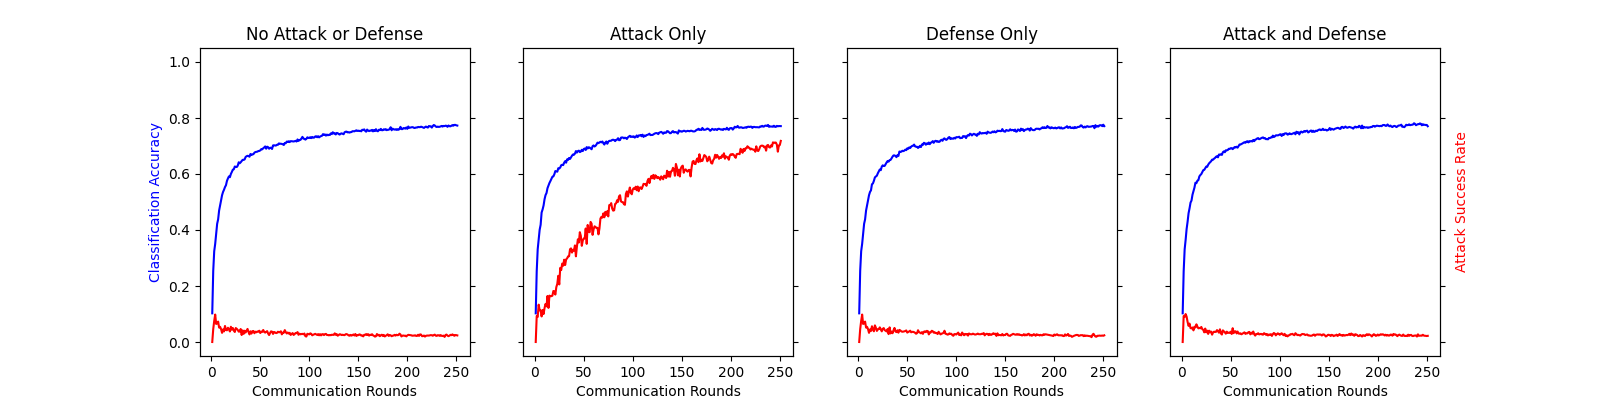
\includegraphics[width=\textwidth]{centralized/alpha10000--alpha_val10000/visuals/accuracy.png}
    \caption{Global Model Performance With Balanced Users and Trusted User}
    \label{fig:accuracy_balanced}
\end{figure}

Figure \ref{fig:threshold_balanced} shows the ability of our threshold to differentiate between benign and malicious user submission. 

\begin{figure}[h!]
    \centering
    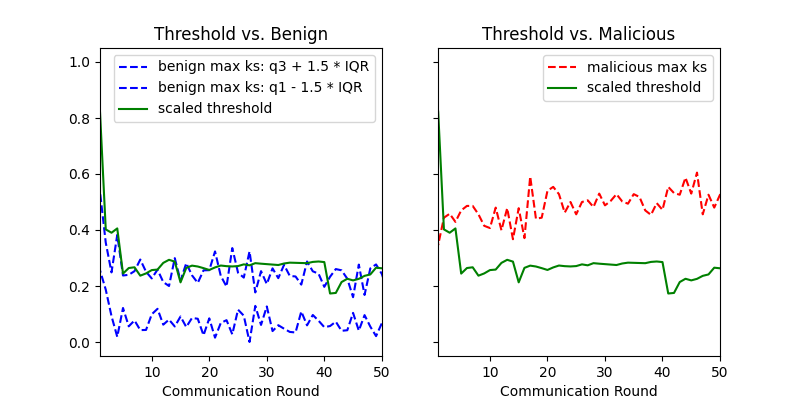
\includegraphics[width=.75\textwidth]{centralized/alpha10000--alpha_val10000/visuals/threshold--d_rounds50.png}
    \caption{Threshold Performance With Balanced Users and Trusted User}
    \label{fig:threshold_balanced}
\end{figure}



% 
\section{Conclusion}

%
\bibliography{iclr2023_conference}
\bibliographystyle{iclr2023_conference}

%
\appendix
\section{Appendix}
You may include other additional sections here.

\end{document}
